\chapter{Getting and installing MongoDB}


Go to \url{http://www.mongodb.org/downloads} and select our OS version. Download it and decompress. Supposing we are in a Linux box and that we are using the latest release (in June 2013) execute the following command: \begin{verbatim}./mongod --rest --dbpath /opt/mongodb-linux-i686-2.4.5/bin/data/db/ \end{verbatim} The server is now listening and waiting for connections, by default, in port 27017. As we have used the \textit{--rest} modifier, we can point our browser to \url{http://localhost:28017} for http diagnostic access. \newline

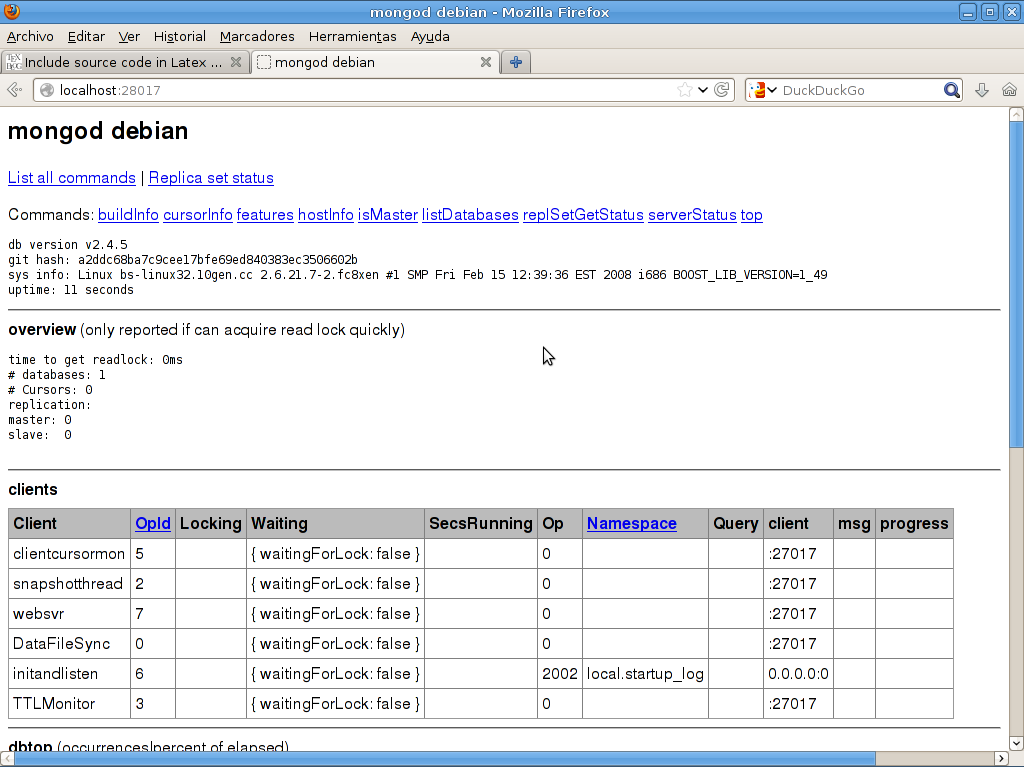
\includegraphics[height=8cm]{images/mongo_webconsole.png}